\section{Introduction}
\begin{frame}
  \frametitle{Introduction}
  \begin{enumerate}
    \item Simulations
    \begin{enumerate}
      \item Created by natural and social scientists
      \item Run on HPC systems
    \end{enumerate}
    \item Real World Systems
    \begin{enumerate}
      \item Massive scale
      \item Inherently concurrent
    \end{enumerate}
    \item Languages
    \begin{enumerate}
      \item C
      \item Fortran
    \end{enumerate}
  \end{enumerate}
\end{frame}

\section{Concurrency}
\subsection{The Actor Model}
\begin{frame}
  \frametitle{The Actor Model}
  \begin{enumerate}
    \item Inherently concurrent
    \item State
    \begin{enumerate}
      \item Isolated
    \end{enumerate}
    \item Communication
    \begin{enumerate}
      \item Message passing
      \item Asynchronous
      \item Reactive
    \end{enumerate}
  \end{enumerate}
  \begin{figure}[htbp]
  \centering
  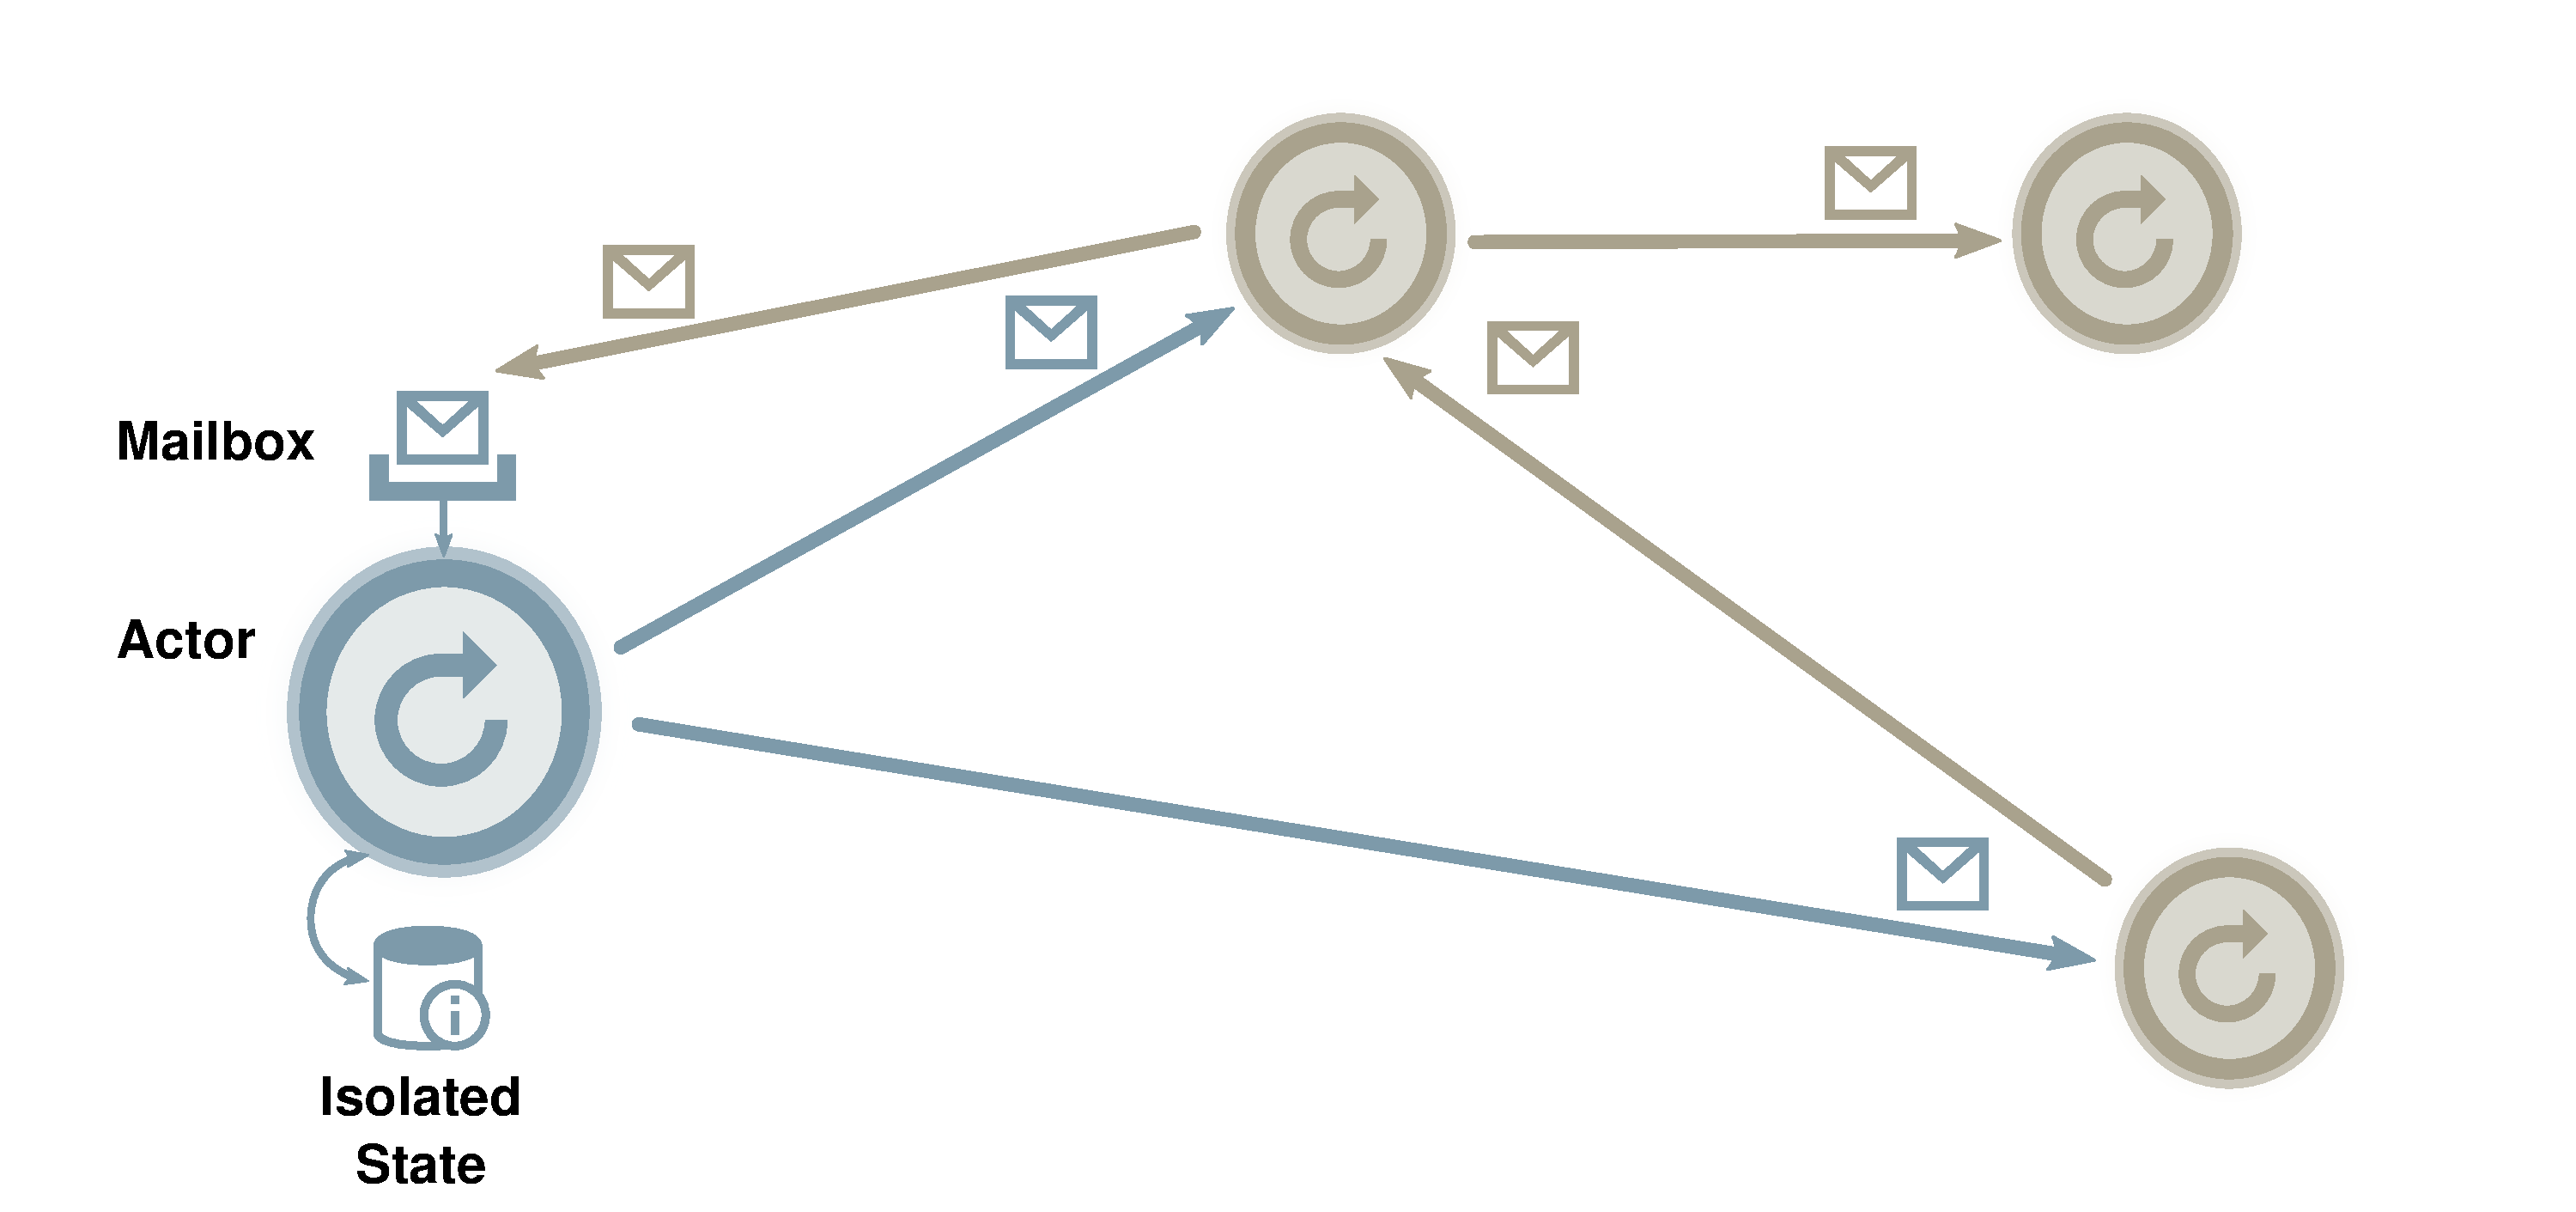
\includegraphics[width=\textwidth]{Images/actors.pdf}
\end{figure}
\end{frame}

\subsection{Message Passing}
\begin{frame}
  \frametitle{Message Passing}
  \begin{enumerate}
    \item Sending
    \begin{enumerate}
      \item Blocking
      \item Non-blocking
    \end{enumerate}
    \item Receiving
    \item MPI
  \end{enumerate}
\end{frame}
